\PassOptionsToPackage{usenames,dvipsnames}{xcolor}
%\documentclass[amsmath,table,sans,amsfonts, handout]{beamer}
\documentclass[amsmath,table,sans,amsfonts,hyperref={colorlinks,citecolor=blue,linkcolor=blue,urlcolor=purple}]{beamer}
\usepackage[T1]{fontenc}
%%\usepackage{beamerthemeshadow}
%%\usepackage[headheight=1pt,footheight=10pt]{beamerthemeboxes}
%%\addfootboxtemplate{\color{structure!80}}{\color{white}\tiny \hfill Karl Svozil (TU Vienna)\hfill}
%%\addfootboxtemplate{\color{structure!65}}{\color{white}\tiny \hfill mur.sat \hfill}
%%\addfootboxtemplate{\color{structure!50}}{\color{white}\tiny \hfill Graz, 2010-12-11\hfill}
%\usepackage[dark]{beamerthemesidebar}
%\usepackage[headheight=24pt,footheight=12pt]{beamerthemesplit}
%\usepackage{beamerthemesplit}
%\usepackage[bar]{beamerthemetree}
\usepackage{graphicx}
\usepackage{pgf}
%\usepackage{eepic}
%\newcommand{\Red}{\color{Red}}  %(VERY-Approx.PANTONE-RED)
%\newcommand{\Green}{\color{Green}}  %(VERY-Approx.PANTONE-GREEN)

\definecolor{applegreen}{rgb}{0.55, 0.71, 0.0}

\usepackage{fourier-orns}  %fancy symbols https://mirror.easyname.at/ctan/fonts/fourier-GUT/doc/fourier-orns-doc.pdf

%\usepackage{musixtex}

\newcommand{\Abschnitt}[1]{{\section #1}}

%%%%%%%%%%%%%%%%%%%%%%%%%%%%%
\usepackage{iftex}
\ifxetex
\usepackage{fontspec}% Schriftumschaltung mit den nativen XeTeX-Anweisungen
                     % vornehmen. Voreinstellung: Latin Modern
%\usepackage[ngerman]{babel}% Sprachumschaltung: Deutsch nach neuer Rechtschreibung



%
% XeLaTeX
%
\XeTeXinputencoding cp1252
\usepackage{fontspec}
%%\setmainfont{Times New Roman}
\setmainfont{Garamond}
\setsansfont{Garamond}
%\setmainfont{EB Garamond}
%\setsansfont{EB Garamond}
%
\else
\usepackage[latin1]{inputenc}
\usepackage[T1]{fontenc}
\fi
%%%%%%%%%%%%%%%%%%%%%%%%%%%%%

%\RequirePackage[german]{babel}
%\selectlanguage{german}
%\RequirePackage[isolatin]{inputenc}

%\pgfdeclareimage[height=0.5cm]{logo}{tu-logo}
%\logo{\pgfuseimage{logo}}
\beamertemplatetriangleitem
%\beamertemplateballitem

\beamerboxesdeclarecolorscheme{alert}{red}{red!15!averagebackgroundcolor}
%\begin{beamerboxesrounded}[scheme=alert,shadow=true]{}
%\end{beamerboxesrounded}

%\beamersetaveragebackground{yellow!10}

%\beamertemplatecircleminiframe

\newtheorem{question}{Question}
\newtheorem{conjecture}[question]{Principle}
\newtheorem{challenge}[question]{Challenge}
\usepackage{tikz}
\newcommand{\bra}[1]{\left< #1 \right|}
\newcommand{\ket}[1]{\left| #1 \right>}

\newcommand{\iprod}[2]{\langle #1 | #2 \rangle}
\newcommand{\mprod}[3]{\langle #1 | #2 | #3 \rangle}
\newcommand{\oprod}[2]{| #1 \rangle\langle #2 |}

\newcommand{\proj}[3]{\begin{smallmatrix} #1 & #2 & #3 \end{smallmatrix}}
\newcommand{\projbf}[3]{\begin{smallmatrix} \mathbf{#1} & \mathbf{#2} & \mathbf{#3} \end{smallmatrix}}

\sloppy
\parskip .7em %vskip between paragraphs

\newcommand{\seq}[1]{\mathbf{#1}}
\newcommand{\floor}[1]{\left\lfloor #1 \right\rfloor}
\newcommand{\ceil}[1]{\left\lceil #1 \right\rceil}
\newcommand{\m}[1]{\widetilde{#1}}
%\newcommand{\p}[1]{\scriptsize\textcolor{black}{$[#1]$}}

\usepackage[most]{tcolorbox}
\begin{document}

\title{\textcolor{blue}{\bf Extending Kolmogorov's axioms for collections of contexts}}
\subtitle{\footnotesize \url{http://tph.tuwien.ac.at/~svozil/publ/2022-QIP22-pres.pdf}
\\
\footnotesize based on \href{https://arxiv.org/abs/1903.10424}{arXiv:1903.10424}}
\author{\textcolor{blue}{Karl Svozil}}
\institute{\normalsize \textcolor{blue}{Institute for theoretical Physics, TU Wien}\\
\textcolor{blue}{svozil@tuwien.ac.at}
%{\tiny Disclaimer: Die hier vertretenen Meinungen des Autors verstehen sich als Diskussionsbeitr�ge und decken sich nicht notwendigerweise mit den Positionen der Technischen Universit�t Wien oder deren Vertreter.}
}
\date{{\color{purple}Tuesday, June 14, 2022, Quantum Information and Probability: From Foundations to Engineering (QIP22)}}
\maketitle


% \frame{
% \frametitle{Contents}
% \tableofcontents
% }

\section{Challenge: Find a True-Implies-False gadget with ``aperture'' $\pi/2$}

\frame{
 \frametitle{Challenge (spontaneous \& unrelated to main topic of talk): Find a True-Implies-False (TIFS) gadget with ``aperture'' $\pi /2$}

 {\color{black}
In 1965 Kochen \& Specker introduced the ``Specker bug'' gadget graph in
}
\href{https://doi.org/10.1007/978-3-0348-9259-9\_19}{DOI 10.1007/978-3-0348-9259-9\_19}.

{\color{black}  In their better known 1967 paper}
\href{https://doi.org/10.1512/iumj.1968.17.17004}{DOI 10.1512/iumj.1968.17.17004}
{\color{black}  they used the ``Specker bug'' gadget to construct a
True-Implies-True (TITS) gadget.

They employed the latter in proofs of
(i) ``the Kochen \& Specker theorem'', as well as a
(ii) configuration of quantum observables that cannot be separated by classical means (ie, two-valued states), indicating non-imbeddibility,
a very strong form of ``contextuality''.

(Subsequently this ``Specker bug'' has been independently re-discovered a couple of times.)
}

}


\frame{
 \frametitle{Challenge (spontaneous \& unrelated to main topic of talk): Find a True-Implies-False (TIFS) gadget with ``aperture'' $\pi /2$ cntd.}

 {\color{black}
For all True-Implies-False gadgets known so far---eg, reviewed in}
\begin{itemize}
\item[$\bullet$]
\href{https://doi.org/10.1103/PhysRevA.98.012106}{Cabello, Portillo, Sol\'{i}s  and KS, DOI 10.1103/PhysRevA.98.012106},\\
\item[$\bullet$]
\href{https://doi.org/10.1063/1.4931658}{Abbott, Calude and KS, DOI 10.1063/1.4931658},\\
\item[$\bullet$]
\href{https://doi.org/10.22331/q-2020-08-14-308}{Ramanathan, Rosicka, Pironio, Karol,  Michal, and Pawel Horodecki, DOI 10.22331/q-2020-08-14-308},\\
\end{itemize}
{\color{black}  the TIFS ``aperture'' beween its end points is less than $\pi /2$.

(TITS with ``aperture'' $\pi /2$ exist plentiful ``by serial composition'' and are used in proofs of ``the Kochen \& Specker theorem''.)
}

}


\frame{
 \frametitle{Challenge (spontaneous \& unrelated to main topic of talk): Find a True-Implies-False (TIFS) gadget with ``aperture'' $\pi /2$ cntd.}

 {\color{black}
Challenge of
Mohammad H. Shekarriz and KS, ``Noncontextual coloring of orthogonality hypergraphs'', Journal of Mathematical Physics 63 (3), 032104 (2022)}
\href{https://doi.org/10.1063/5.0062801}{DOI 10.1063/5.0062801}{\color{purple}:}
\begin{center}
{\large \bf \color{purple} ``Find a TIFS containing no TITS as subgadget whose ``aperture'' is exactly $\pi /2$.\\Or, alternatively, prove that this is impossible.''}
\end{center}

ps: trivial TIFS like a single context---there should at least be two intertwining contexts, or TITS-TIFS combos, are excluded.

pps: Any proof that a faithful orthogonal representation of a TIFS with aperture $\pi /2$ might ultimately require geometric means. Maybe such a proof is elementary or hard, I have not intuition about it.

}


%%%%%%%%%%%%%%%%%%%%%%%%%%%%%%%%%%%%%%%%%%%%%%%%%%%%%%%%%%%%%%%%%%%%%%%%%%%%%%%%%%%%%%%%%%%%%%%%%%%%%%%%%%%%%%%%%%%%%%%%%%%%%%%%%%%%%%%%%%%%%
%%%%%%%%%%%%%%%%%%%%%%%%%%%%%%%%%%%%%%%%%%%%%%%%%%%%%%%%%%%%%%%%%%%%%%%%%%%%%%%%%%%%%%%%%%%%%%%%%%%%%%%%%%%%%%%%%%%%%%%%%%%%%%%%%%%%%%%%%%%%%
%%%%%%%%%%%%%%%%%%%%%%%%%%%%%%%%%%%%%%%%%%%%%%%%%%%%%%%%%%%%%%%%%%%%%%%%%%%%%%%%%%%%%%%%%%%%%%%%%%%%%%%%%%%%%%%%%%%%%%%%%%%%%%%%%%%%%%%%%%%%%
%%%%%%%%%%%%%%%%%%%%%%%%%%%%%%%%%%%%%%%%%%%%%%%%%%%%%%%%%%%%%%%%%%%%%%%%%%%%%%%%%%%%%%%%%%%%%%%%%%%%%%%%%%%%%%%%%%%%%%%%%%%%%%%%%%%%%%%%%%%%%
%%%%%%%%%%%%%%%%%%%%%%%%%%%%%%%%%%%%%%%%%%%%%%%%%%%%%%%%%%%%%%%%%%%%%%%%%%%%%%%%%%%%%%%%%%%%%%%%%%%%%%%%%%%%%%%%%%%%%%%%%%%%%%%%%%%%%%%%%%%%%


\section{Category formation by different views on the same physical entity in the presence of complementarity}

\begin{frame}[shrink=1.2]
 \frametitle{Category formation by different views on the same physical entity in the presence of complementarity}

\begin{itemize}
\item[$\bullet$] {
%\color{purple}
Schr\"odinger, on p.~15~of ``My View of the World'', quoted the Vedantic analogy of a
{\color{purple} \em ``many-faceted crystal which, while showing hundreds of little
pictures of what is in reality a single existent object, does
not really multiply that object. $\ldots$ A comparison used in Hinduism is of the
many almost identical images which a many-faceted
diamond makes of some one object such as the sun.''} }
\pause
\item[$\bullet$] {
%\color{purple}
An example is the coordinatization or coding and encryption of a vector relative to and ``viewed from'' different bases.
}
\pause
\item[$\bullet$] {
%\color{purple}
Another example from partition logic---aka automaton logik aka Wright's generalized urn model:
the different ``ball states'' (aka partitions referring to collections of ball types) when ``viewed by different color filters''.
}
\pause
\item[$\bullet$] {
%\color{purple}
This is about epistemology,
since either the ontology ``remains hidden'' as it cannot be accessed by physical means in the presence of complementarity,
or is restricted to merely one maximal observable aka context.
}
\end{itemize}
\end{frame}

\frame{
\frametitle{Informal notion of maximal observables aka contexts}

A ``view'' or (used synonymously)  ``frame'' or ``context''  will be in full generality and thus informally (glancing at heuristics from quantum mechanics and partition logic)
characterized as some domain or set of observables or properties
which are
\begin{itemize}
\item[(i)]
{\em largest} or {\em maximal} in the sense that any extension yields redundancies,
\item[(ii)]
yet at the same time in the {\em finest resolution} in the sense that the respective observables or properties are ``no composite'' of ``more elementary'' ones,
\item[(iii)]
{\em mutually exclusive} in the sense that one property or observation excludes another, different property or observation, as well as
\item[(iv)]
contains only {\em simultaneously measurable, compatible} observables or properties.
\end{itemize}

}

\section{Generalization of Kolmogorov's axioms to arbitrary event structures}


\frame{
\frametitle{Generalization of Kolmogorov's axioms to arbitrary event structures}

Suppose two arbitrary contexts
${\cal C}_1=\{ {\bf e}_1, \ldots {\bf e}_n \}$
and
${\cal C}_2=\{ {\bf f}_1, \ldots {\bf f}_m \}$.
The conditional probabilities
$P( {\bf f}_j \vert {\bf e}_i )$, with $1 \le j \le m$ and $1 \le i \le n$, which
alternatively can be considered as
either measuring the Bayesian degree of reasonable expectation representing
a state of knowledge or as quantification of a personal belief
or the frequency of occurrence
of ``${\bf f}_j$ given ${\bf e}_i$'',
can be arranged into a $(n \times m)$-matrix whose entries are $P( {\bf f}_j \vert {\bf e}_i )$, that is,
\begin{equation}
\begin{split}
\left[ P( {\cal C}_2 \vert {\cal C}_1 )\right] =
\left[ P( \{{\bf f}_1, \ldots {\bf f}_m  \} \vert \{ {\bf e}_1, \ldots {\bf e}_n \} ) \right]
\\
\equiv
\begin{bmatrix}
{P({\bf f}_1 \vert  {\bf e}_1)}  & \cdots & {P({\bf f}_m \vert  {\bf e}_1)}      \\
 \cdots &  \cdots &  \cdots \\
{P({\bf f}_1 \vert  {\bf e}_n)}  & \cdots &   {P({\bf f}_m \vert  {\bf e}_n)}
\end{bmatrix}
.
\end{split}
\label{2020-k-gka}
\end{equation}

}

\frame{
\frametitle{Generalization of Kolmogorov's axioms to arbitrary event structures cntd.}

Assume that the conditional probabilities of the elements of the second context with respect to
an arbitrary element ${\bf e}_k\in  {\cal C}_1$ of the first context ${\cal C}_1$
are non-negative, additive, and that, if this sum is extended over the entire second context ${\cal C}_2$,
it adds up to one:
\begin{equation}
\begin{split}
P({\bf f}_i \vert  {\bf e}_k) + P({\bf f}_j \vert  {\bf e}_k)
=
P[(  {\bf f}_i \cup {\bf f}_j  ) \vert  {\bf e}_k]
\\
\sum_{{\bf f}_i \in  {\cal C}_2}  P({\bf f}_i \vert  {\bf e}_k) = P\left[\left(\bigcup_{{\bf f}_i \in  {\cal C}_2}  {\bf f}_i \right) \vert  {\bf e}_k\right]  = 1
.
\end{split}
\label{2020-k-gka12}
\end{equation}
That is,  the row sum taken within every single row of $\left[ P( {\cal C}_2 \vert {\cal C}_1 )\right]$ adds up to one.

This generalises Kolmogorov's axioms as it allows cases in which both contexts do not coincide.

}


\section{Examples: Quantum bistochasticity}

\frame{
 \frametitle{Examples: Quantum bistochasticity}

The multi-context quantum case has been studied in great detail with  emphasis on motivating and deriving the
Born rule from elementary foundations by Alexia Auff\'eves  and Philippe Grangier, eg (among others),
\begin{itemize}
\item[$\bullet$]  \href{https://doi.org/10.1038/srep43365}{DOI 10.1038/srep43365}
\item[$\bullet$]  \href{https://doi.org/10.1098/rsta.2017.0311}{DOI 10.1098/rsta.2017.0311}
\end{itemize}

Please look at their papers!


}

\section{Examples: Two intertwining three-atomic contexts---the ``firefly'' logic}

\begin{frame}[shrink=1.4]
 \frametitle{Examples: Two intertwining three-atomic contexts---the ``firefly'' logic $L_{12}$}
{\scriptsize
Hypergraph of  the $L_{12}$ ``firefly'' logic.
(a) The associated (quasi)classical partition logic representation
obtained through in inverse construction using all two-valued measures thereon;
(b) a faithful orthogonal representation
rendering a quantum {\it double};
(c) ``classical'' two-valued measure number $1$;
(d) a pure quantum state prepared as $\begin{pmatrix}1,0,0\end{pmatrix}^\intercal$.
A red square and gray and green circles indicate value assignments $1$, $\frac{1}{2}$ and $0$, respectively.}

\begin{center}
\begin{tabular}{cc}
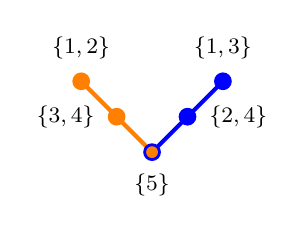
\begin{tikzpicture}  [scale=0.15]

\newdimen\ms
\ms=0.05cm

\tikzstyle{every path}=[line width=1.5pt]

\tikzstyle{c3}=[circle,inner sep={\ms/8},minimum size=4.5*\ms]
\tikzstyle{c2}=[circle,inner sep={\ms/8},minimum size=3*\ms]
\tikzstyle{c1}=[circle,inner sep={\ms/8},minimum size=1.5*\ms]

% Radius of regular polygons
\newdimen\R
\R=6cm     % outer circle

%\r= { \R * sqrt(3) }     % inner circle
%\newdimen\r
%\r=    {\R * sqrt(3)/2}       % inner circle

%\newdimen\K
%\K=3cm

% Define positions of all observables
\path
  (0,6 ) coordinate(1)
  (3,3    ) coordinate(2)
  (6,0 ) coordinate(3)
  (9,3) coordinate(4)
  (12,6  ) coordinate(5)
;

% draw contexts

\draw [color=orange] (1) -- (2) -- (3);
\draw [color=blue] (3) -- (4) -- (5);


%
%%
%% draw atoms
%%
%
\draw (1) coordinate[c3,fill=orange,label={above:\footnotesize $\{1,2\}$}];   %
%
\draw (2) coordinate[c3,fill=orange,label={left:\footnotesize $\{3,4\}$}];    %
%
\draw (3) coordinate[c3,fill=blue,label={below:\footnotesize $\{5\}$}]; %
\draw (3) coordinate[c2,fill=orange];  %
%
\draw (4) coordinate[c3,fill=blue,label={right:\footnotesize $\{2,4\}$}];  %
%
\draw (5) coordinate[c3,fill=blue,label={above:\footnotesize $\{1,3\}$}];  %
%
%

\end{tikzpicture}
&
\begin{tikzpicture}  [scale=0.15]

\newdimen\ms
\ms=0.05cm

\tikzstyle{every path}=[line width=1.5pt]

\tikzstyle{c3}=[circle,inner sep={\ms/8},minimum size=4.5*\ms]
\tikzstyle{c2}=[circle,inner sep={\ms/8},minimum size=3*\ms]
\tikzstyle{c1}=[circle,inner sep={\ms/8},minimum size=1.5*\ms]

% Radius of regular polygons
\newdimen\R
\R=6cm     % outer circle

%\r= { \R * sqrt(3) }     % inner circle
%\newdimen\r
%\r=    {\R * sqrt(3)/2}       % inner circle

%\newdimen\K
%\K=3cm

% Define positions of all observables
\path
  (0,6 ) coordinate(1)
  (3,3    ) coordinate(2)
  (6,0 ) coordinate(3)
  (9,3) coordinate(4)
  (12,6  ) coordinate(5)
;

% draw contexts

\draw [color=orange] (1) -- (2) -- (3);
\draw [color=blue] (3) -- (4) -- (5);


%
%%
%% draw atoms
%%
%
\draw (1) coordinate[c3,fill=orange,label={above:\footnotesize $\begin{pmatrix}1,0,0\end{pmatrix}^\intercal$}];   %
%
\draw (2) coordinate[c3,fill=orange,label={left:\footnotesize  $\begin{pmatrix}0,1,0\end{pmatrix}^\intercal$}];    %
%
\draw (3) coordinate[c3,fill=blue,label={below:\footnotesize    $\begin{pmatrix}0,0,1\end{pmatrix}^\intercal$}]; %
\draw (3) coordinate[c2,fill=orange];  %
%
\draw (4) coordinate[c3,fill=blue,label={right:\footnotesize    $\frac{1}{\sqrt{2}}\begin{pmatrix}1,1,0\end{pmatrix}^\intercal$}];  %
%
\draw (5) coordinate[c3,fill=blue,label={above:\footnotesize    $\frac{1}{\sqrt{2}}\begin{pmatrix}1,-1,0\end{pmatrix}^\intercal$}];  %
%
%

\end{tikzpicture}
\\
(a)&(b)
\\
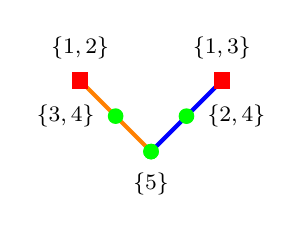
\begin{tikzpicture}  [scale=0.15]

\newdimen\ms
\ms=0.05cm

\tikzstyle{every path}=[line width=1.5pt]

\tikzstyle{s1}=[color=red,inner sep=2,rectangle,minimum size=6]
\tikzstyle{c2}=[circle,inner sep=2,minimum size=4]

% Radius of regular polygons
\newdimen\R
\R=6cm     % outer circle

%\r= { \R * sqrt(3) }     % inner circle
%\newdimen\r
%\r=    {\R * sqrt(3)/2}       % inner circle

%\newdimen\K
%\K=3cm

% Define positions of all observables
\path
  (0,6 ) coordinate(1)
  (3,3    ) coordinate(2)
  (6,0 ) coordinate(3)
  (9,3) coordinate(4)
  (12,6  ) coordinate(5)
;

% draw contexts

\draw [color=orange] (1) -- (2) -- (3);
\draw [color=blue] (3) -- (4) -- (5);


%
%%
%% draw atoms
%%
%
\draw (1) coordinate[s1,fill=red,label={above:\footnotesize $\{1,2\}$}];   %
%
\draw (2) coordinate[c2,fill=green,label={left:\footnotesize $\{3,4\}$}];    %
%
\draw (3) coordinate[c2,fill=green,label={below:\footnotesize $\{5\}$}]; %
\draw (3) coordinate[c2,fill=green];  %
%
\draw (4) coordinate[c2,fill=green,label={right:\footnotesize $\{2,4\}$}];  %
%
\draw (5) coordinate[s1,fill=red,label={above:\footnotesize $\{1,3\}$}];  %
%
%

\end{tikzpicture}
&
\begin{tikzpicture}  [scale=0.15]

\newdimen\ms
\ms=0.05cm

\tikzstyle{every path}=[line width=1.5pt]

\tikzstyle{s1}=[color=red,inner sep=2,rectangle,minimum size=6]
\tikzstyle{c2}=[circle,inner sep=2,minimum size=4]

% Radius of regular polygons
\newdimen\R
\R=6cm     % outer circle

%\r= { \R * sqrt(3) }     % inner circle
%\newdimen\r
%\r=    {\R * sqrt(3)/2}       % inner circle

%\newdimen\K
%\K=3cm

% Define positions of all observables
\path
  (0,6 ) coordinate(1)
  (3,3    ) coordinate(2)
  (6,0 ) coordinate(3)
  (9,3) coordinate(4)
  (12,6  ) coordinate(5)
;

% draw contexts

\draw [color=orange] (1) -- (2) -- (3);
\draw [color=blue] (3) -- (4) -- (5);


%
%%
%% draw atoms
%%
%
\draw (1) coordinate[s1,fill=red,label={above:\footnotesize   $\begin{pmatrix}1,0,0\end{pmatrix}^\intercal$}];   %
%
\draw (2) coordinate[c2,fill=green,label={left:\footnotesize  $\begin{pmatrix}0,1,0\end{pmatrix}^\intercal$}];    %
%
\draw (3) coordinate[c2,fill=green,label={below:\footnotesize $\begin{pmatrix}0,0,1\end{pmatrix}^\intercal$}]; %
\draw (3) coordinate[c2,fill=green];  %
%
\draw (4) coordinate[c2,fill=gray,label={right:\footnotesize  $\frac{1}{\sqrt{2}}\begin{pmatrix}1,1,0\end{pmatrix}^\intercal$}];  %
%
\draw (5) coordinate[c2,fill=gray,label={above:\footnotesize  $\frac{1}{\sqrt{2}}\begin{pmatrix}1,-1,0\end{pmatrix}^\intercal$}];  %
%
%

\end{tikzpicture}
\\
(c)&(d)
\end{tabular}
\end{center}


\end{frame}

\begin{frame}[shrink=1.4]
 \frametitle{Examples: Classical probabilities on two intertwining three-atomic contexts---the ``firefly'' logic $L_{12}$}

The  $L_{12}$ ``firefly'' logic labels the atoms (aka elementary propositions)
obtained by an ``inverse construction''
using all five two-valued measures thereon.
By design, it will be very similar to the earlier logic with four atoms.
With the identifications
${\bf e}_1 \equiv \{1,2\}$,
${\bf e}_2 \equiv \{3,4\}$,
${\bf e}_3 = {\bf f}_3 \equiv \{5\}$,
${\bf f}_1 \equiv \{1,3\}$, and
${\bf f}_2 \equiv \{2,4\}$
we obtain all classical probabilities
by identifying $i \rightarrow \lambda_i > 0$.
The respective conditional probabilities are
\begin{equation}
\begin{split}
\left[ P( {\cal C}_2 \vert {\cal C}_1 )\right] =
\left[ P( \{ {\bf f}_1, {\bf f}_2, {\bf f}_3 \} \vert \{ {\bf e}_1,{\bf e}_2,{\bf e}_3 \} ) \right]
\\
\equiv
%\begin{bmatrix}
%{P({\bf f}_1 \vert  {\bf e}_1)}  &  {P({\bf f}_2 \vert  {\bf e}_1)}   & {P({\bf f}_3 \vert  {\bf e}_1)}    \\
%{P({\bf f}_1 \vert  {\bf e}_2)}  &  {P({\bf f}_2 \vert  {\bf e}_2)}   & {P({\bf f}_3 \vert  {\bf e}_2)}    \\
%{P({\bf f}_1 \vert  {\bf e}_3)}  &  {P({\bf f}_2 \vert  {\bf e}_3)}   & {P({\bf f}_3 \vert  {\bf e}_3)}
%\end{bmatrix}
%\\
%=
%\begin{bmatrix}
%\frac{P({\bf f}_1 \cap {\bf e}_1)}{P({\bf e}_1)}  &  \frac{P({\bf f}_2 \cap {\bf e}_1)}{P({\bf e}_1)}   & \frac{P({\bf f}_3 \cap {\bf e}_1)}{P({\bf e}_1)}    \\
%\frac{P({\bf f}_1 \cap {\bf e}_2)}{P({\bf e}_2)}  &  \frac{P({\bf f}_2 \cap {\bf e}_2)}{P({\bf e}_2)}   & \frac{P({\bf f}_3 \cap {\bf e}_2)}{P({\bf e}_2)}    \\
%\frac{P({\bf f}_1 \cap {\bf e}_3)}{P({\bf e}_3)}  &  \frac{P({\bf f}_2 \cap {\bf e}_3)}{P({\bf e}_3)}   & \frac{P({\bf f}_3 \cap {\bf e}_3)}{P({\bf e}_3)}
%\end{bmatrix}
%\\
%=
%\begin{bmatrix}
%\frac{P( \{1,3\}  \cap  \{1,2\} )}{P( \{1,2\} )}  &  \frac{P( \{2,4\}  \cap  \{1,2\} )}{P( \{1,2\} )}   & \frac{P( \{5\}  \cap  \{1,2\} )}{P( \{1,2\} )}    \\
%\frac{P( \{1,3\}  \cap  \{3,4\} )}{P( \{3,4\} )}  &  \frac{P( \{2,4\}  \cap  \{3,4\} )}{P( \{3,4\} )}   & \frac{P( \{5\}  \cap  \{3,4\} )}{P( \{3,4\} )}    \\
%\frac{P( \{1,3\}  \cap  \{5\} )}{P( \{5\} )}  &  \frac{P( \{2,4\}  \cap  \{5\} )}{P( \{5\} )}   & \frac{P( \{5\}  \cap  \{5\} )}{P( \{5\} )}
%\end{bmatrix}
%\\
%=
\begin{bmatrix}
\frac{P( \{1\} )}{P( \{1,2\} )}  &  \frac{P( \{2\} )}{P( \{1,2\} )}   & \frac{P( \emptyset )}{P( \{1,2\} )}    \\
\frac{P( \{3\} )}{P( \{3,4\} )}  &  \frac{P( \{4\} )}{P( \{3,4\} )}   & \frac{P( \emptyset  )}{P( \{3,4\} )}    \\
\frac{P( \emptyset  )}{P( \{5\} )}  &  \frac{P( \emptyset  )}{P( \{5\} )}   & \frac{P( \{5\} )}{P( \{5\} )}
\end{bmatrix}
=
\begin{bmatrix}
\frac{ \lambda_1 }{ \lambda_1+\lambda_2 }  &  \frac{ \lambda_2 }{ \lambda_1+\lambda_2 }   & 0    \\
\frac{ \lambda_3 }{ \lambda_3+\lambda_4 }  &  \frac{ \lambda_4 }{ \lambda_3+\lambda_4 }   & 0    \\
0  &  0   & 1
\end{bmatrix},
\end{split}
\end{equation}
as well as
\begin{equation}
\begin{split}
\left[ P( {\cal C}_1 \vert {\cal C}_2 )\right] =
\left[ P( \{ {\bf e}_1, {\bf e}_2, {\bf e}_3 \} \vert \{ {\bf f}_1,{\bf f}_2,{\bf f}_3 \} ) \right]
\\
\equiv
%\begin{bmatrix}
%{P({\bf e}_1 \vert  {\bf f}_1)}  &  {P({\bf e}_2 \vert  {\bf f}_1)}   & {P({\bf e}_3 \vert  {\bf f}_1)}    \\
%{P({\bf e}_1 \vert  {\bf f}_2)}  &  {P({\bf e}_2 \vert  {\bf f}_2)}   & {P({\bf e}_3 \vert  {\bf f}_2)}    \\
%{P({\bf e}_1 \vert  {\bf f}_3)}  &  {P({\bf e}_2 \vert  {\bf f}_3)}   & {P({\bf e}_3 \vert  {\bf f}_3)}
%\end{bmatrix}
%\\
%=
%\begin{bmatrix}
%\frac{P({\bf e}_1 \cap {\bf f}_1)}{P({\bf f}_1)}  &  \frac{P({\bf e}_2 \cap {\bf f}_1)}{P({\bf f}_1)}   & \frac{P({\bf e}_3 \cap {\bf f}_1)}{P({\bf f}_1)}    \\
%\frac{P({\bf e}_1 \cap {\bf f}_2)}{P({\bf f}_2)}  &  \frac{P({\bf e}_2 \cap {\bf f}_2)}{P({\bf f}_2)}   & \frac{P({\bf e}_3 \cap {\bf f}_2)}{P({\bf f}_2)}    \\
%\frac{P({\bf e}_1 \cap {\bf f}_3)}{P({\bf f}_3)}  &  \frac{P({\bf e}_2 \cap {\bf f}_3)}{P({\bf f}_3)}   & \frac{P({\bf e}_3 \cap {\bf f}_3)}{P({\bf f}_3)}
%\end{bmatrix}
%\\
%=
%\begin{bmatrix}
%\frac{P( \{1,2\}  \cap  \{1,3\} )}{P( \{1,3\} )}  &  \frac{P( \{3,4\}  \cap  \{1,3\} )}{P( \{1,3\} )}   & \frac{P( \{5\}  \cap  \{1,3\} )}{P( \{1,3\} )}    \\
%\frac{P( \{1,2\}  \cap  \{2,4\} )}{P( \{2,4\} )}  &  \frac{P( \{3,4\}  \cap  \{2,4\} )}{P( \{2,4\} )}   & \frac{P( \{5\}  \cap  \{2,4\} )}{P( \{2,4\} )}    \\
%\frac{P( \{1,2\}  \cap  \{5\} )}{P( \{5\} )}  &  \frac{P( \{3,4\}  \cap  \{5\} )}{P( \{5\} )}   & \frac{P( \{5\}  \cap  \{5\} )}{P( \{5\} )}
%\end{bmatrix}
%\\
%=
\begin{bmatrix}
\frac{P( \{1\} )}{P( \{1,3\} )}  &  \frac{P( \{3\} )}{P( \{1,3\} )}   & \frac{P( \emptyset )}{P( \{1,3\} )}    \\
\frac{P( \{2\} )}{P( \{2,4\} )}  &  \frac{P( \{4\} )}{P( \{2,4\} )}   & \frac{P( \emptyset  )}{P( \{2,4\} )}    \\
\frac{P( \emptyset  )}{P( \{5\} )}  &  \frac{P( \emptyset  )}{P( \{5\} )}   & \frac{P( \{5\} )}{P( \{5\} )}
\end{bmatrix}
=
\begin{bmatrix}
\frac{ \lambda_1 }{ \lambda_1+\lambda_3 }  &  \frac{ \lambda_3 }{ \lambda_1+\lambda_3 }   & 0    \\
\frac{ \lambda_2 }{ \lambda_2+\lambda_4 }  &  \frac{ \lambda_4 }{ \lambda_2+\lambda_4 }   & 0    \\
0  &  0   & 1
\end{bmatrix}
.
\end{split}
\label{2019-k-e-fireflyrsm}
\end{equation}

\end{frame}

\section{Examples: classical probabilities on House/Pentagon/Pentagram hyperdiagram}

\frame{
 \frametitle{Examples: classical probabilities on House/Pentagon/Pentagram hyperdiagram}

Hypergraph of the pentagon/pentagram/house logic with partition logic labelling (also available: vertex labelling by vectors aka faithful orthogonal representations).

\begin{center}
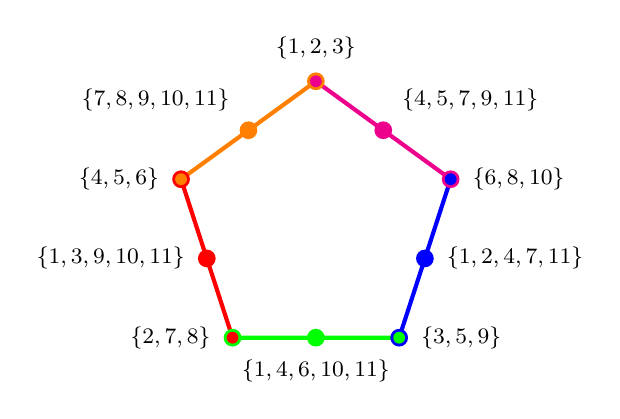
\begin{tikzpicture}  [scale=0.3]

\newdimen\ms
\ms=0.05cm

\tikzstyle{every path}=[line width=1.5pt]

\tikzstyle{c3}=[circle,inner sep={\ms/8},minimum size=4.5*\ms]
\tikzstyle{c2}=[circle,inner sep={\ms/8},minimum size=3*\ms]
\tikzstyle{c1}=[circle,inner sep={\ms/8},minimum size=1.5*\ms]

% Radius of regular polygons
\newdimen\R
\R=6cm     % outer circle

%\r= { \R * sqrt(3) }     % inner circle
%\newdimen\r
%\r=    {\R * sqrt(3)/2}       % inner circle

%\newdimen\K
%\K=3cm

% Define positions of all observables
\path
  ({90 + 0 * 360 /5}:\R      ) coordinate(1)
  ({90 + 36 + 0 * 360 /5}:{\R * sqrt((25+10*sqrt(5))/(50+10*sqrt(5)))}      ) coordinate(2)
  ({90 + 1 * 360 /5}:\R   ) coordinate(3)
  ({90 + 36 + 1 * 360 /5}:{\R * sqrt((25+10*sqrt(5))/(50+10*sqrt(5)))}   ) coordinate(4)
  ({90 + 2 * 360 /5}:\R  ) coordinate(5)
  ({90 + 36 + 2 * 360 /5}:{\R * sqrt((25+10*sqrt(5))/(50+10*sqrt(5)))}  ) coordinate(6)
  ({90 + 3 * 360 /5}:\R  ) coordinate(7)
  ({90 + 36 + 3 * 360 /5}:{\R * sqrt((25+10*sqrt(5))/(50+10*sqrt(5)))}  ) coordinate(8)
  ({90 + 4 * 360 /5}:\R     ) coordinate(9)
  ({90 + 36 + 4 * 360 /5}:{\R * sqrt((25+10*sqrt(5))/(50+10*sqrt(5)))}     ) coordinate(10)
;

% draw contexts

\draw [color=orange] (1) -- (2) -- (3);
\draw [color=red] (3) -- (4) -- (5);
\draw [color=green] (5) -- (6) -- (7);
\draw [color=blue] (7) -- (8) -- (9);
\draw [color=magenta] (9) -- (10) -- (1);    %


%
%%
%% draw atoms
%%
%
\draw (1) coordinate[c3,fill=orange,label=90:{\footnotesize $\{ 1,2,3\} $}];   %
\draw (1) coordinate[c2,fill=magenta];  %
%
\draw (2) coordinate[c3,fill=orange,label={above left:\footnotesize $\{ 7,8,9,10,11\}$}];    %
%
\draw (3) coordinate[c3,fill=red,label={left:\footnotesize $\{ 4,5,6\} $}]; %
\draw (3) coordinate[c2,fill=orange];  %
%
\draw (4) coordinate[c3,fill=red,label={left:\footnotesize $\{ 1,3,9,10,11\}$}];  %
%
\draw (5) coordinate[c3,fill=green,label={left:\footnotesize $\{ 2,7,8\} $}];  %
\draw (5) coordinate[c2,fill=red];  %
%
\draw (6) coordinate[c3,fill=green,label={below:\footnotesize $\{ 1,4,6,10,11\} $}];
%
\draw (7) coordinate[c3,fill=blue,label={right:\footnotesize $\{ 3,5,9\}$}];  %
\draw (7) coordinate[c2,fill=green];  %
%
\draw (8) coordinate[c3,fill=blue,label={right:\footnotesize $\{ 1,2,4,7,11\}$}];  %
%
\draw (9) coordinate[c3,fill=magenta,label={right:\footnotesize $\{ 6,8,10\}$}];
\draw (9) coordinate[c2,fill=blue];  %
%
\draw (10) coordinate[c3,fill=magenta,label={above right:\footnotesize $\{ 4,5,7,9,11\}$}];  %
%
%
\end{tikzpicture}
\end{center}

}

\section{Examples: classical probabilities on House/Pentagon/Pentagram hyperdiagram}

\begin{frame}[shrink=1.4]
 \frametitle{Examples: classical probabilities on House/Pentagon/Pentagram hyperdiagram cntd.}

With the identifications
${\bf e}_1 \equiv \{1,2,3\}$,
${\bf e}_2 \equiv \{4,5,7,9,11\}$,
${\bf e}_3   \equiv \{6,8,10\}$,
${\bf f}_1 \equiv \{2,7,8\}$,
${\bf f}_2 \equiv \{1,3,9,10,11\}$, and
${\bf f}_3   \equiv \{4,5,6\}$.
The respective conditional probabilities are
\begin{equation}
\begin{split}
\left[ P( {\cal C}_2 \vert {\cal C}_1 )\right] =
\left[ P( \{ {\bf f}_1, {\bf f}_2, {\bf f}_3 \} \vert \{ {\bf e}_1,{\bf e}_2,{\bf e}_3 \} ) \right]
\\
\equiv
%\begin{bmatrix}
%{P({\bf f}_1 \vert  {\bf e}_1)}  &  {P({\bf f}_2 \vert  {\bf e}_1)}   & {P({\bf f}_3 \vert  {\bf e}_1)}    \\
%{P({\bf f}_1 \vert  {\bf e}_2)}  &  {P({\bf f}_2 \vert  {\bf e}_2)}   & {P({\bf f}_3 \vert  {\bf e}_2)}    \\
%{P({\bf f}_1 \vert  {\bf e}_3)}  &  {P({\bf f}_2 \vert  {\bf e}_3)}   & {P({\bf f}_3 \vert  {\bf e}_3)}
%\end{bmatrix}
%=
%\begin{bmatrix}
%\frac{P({\bf f}_1 \cap {\bf e}_1)}{P({\bf e}_1)}  &  \frac{P({\bf f}_2 \cap {\bf e}_1)}{P({\bf e}_1)}   & \frac{P({\bf f}_3 \cap {\bf e}_1)}{P({\bf e}_1)}    \\
%\frac{P({\bf f}_1 \cap {\bf e}_2)}{P({\bf e}_2)}  &  \frac{P({\bf f}_2 \cap {\bf e}_2)}{P({\bf e}_2)}   & \frac{P({\bf f}_3 \cap {\bf e}_2)}{P({\bf e}_2)}    \\
%\frac{P({\bf f}_1 \cap {\bf e}_3)}{P({\bf e}_3)}  &  \frac{P({\bf f}_2 \cap {\bf e}_3)}{P({\bf e}_3)}   & \frac{P({\bf f}_3 \cap {\bf e}_3)}{P({\bf e}_3)}
%\end{bmatrix}
%\\
%=
\begin{bmatrix}
\frac{P( \{2,7,8\}  \cap  \{1,2,3\} )}{P( \{1,2,3\} )} &  \frac{P( \{1,3,9,10,11\}  \cap  \{1,2,3\} )}{P( \{1,2,3\} )} &  \frac{P( \{4,5,6\}  \cap  \{1,2,3\} )}{P( \{1,2,3\} )}    \\
\frac{P( \{2,7,8\}  \cap  \{4,5,7,9,11\} )}{P( \{4,5,7,9,11\} )}  &  \frac{P( \{1,3,9,10,11\}  \cap  \{4,5,7,9,11\} )}{P( \{4,5,7,9,11\} )}   & \frac{P( \{4,5,6\}  \cap  \{4,5,7,9,11\} )}{P( \{4,5,7,9,11\} )}    \\
\frac{P( \{2,7,8\}  \cap  \{6,8,10\} )}{P( \{6,8,10\} )}  &  \frac{P( \{1,3,9,10,11\}  \cap  \{6,8,10\} )}{P( \{6,8,10\} )}   & \frac{P( \{4,5,6\}  \cap  \{6,8,10\} )}{P( \{6,8,10\} )}
\end{bmatrix}
\\
=
\begin{bmatrix}
\frac{P( \{2\} )}{P( \{1,2,3\} )}  &  \frac{P( \{1,3\} )}{P( \{1,2,3\} )}   & \frac{P( \emptyset)}{P( \{1,2,3\} )}    \\
\frac{P( \{7\} )}{P( \{4,5,7,9,11\} )}  &  \frac{P( \{11\} )}{P( \{4,5,7,9,11\} )}   & \frac{P( \{4,5 \} )}{P( \{4,5,7,9,11\} )}    \\
\frac{P( \{8\} )}{P( \{6,8,10\} )}  &  \frac{P( \{10\} )}{P( \{6,8,10\} )}   & \frac{P( \{6\} )}{P( \{6,8,10\} )}
\end{bmatrix}
\\
=
\begin{bmatrix}
\frac{ \lambda_2 }{ \lambda_1+\lambda_2 +\lambda_3}  &  \frac{ \lambda_1 + \lambda_3 }{\lambda_1+\lambda_2 +\lambda_3 }   &  0    \\
\frac{ \lambda_7 }{ \lambda_4+\lambda_5 + \lambda_7+\lambda_9 +\lambda_{11}  }  &  \frac{ \lambda_9 + \lambda_{11}}{ \lambda_4+\lambda_5 + \lambda_7+\lambda_9 +\lambda_{11}  }   & \frac{ \lambda_4+\lambda_5 }{ \lambda_4+\lambda_5 + \lambda_7+\lambda_9 +\lambda_{11}  }     \\
\frac{ \lambda_8 }{ \lambda_6+\lambda_8+\lambda_{10} }  &  \frac{ \lambda_{10} }{ \lambda_6+\lambda_8+\lambda_{10} }   & \frac{ \lambda_6 }{ \lambda_6+\lambda_8+\lambda_{10} }
\end{bmatrix}.
\end{split}
\end{equation}

\end{frame}

\section{Examples: ``exotic'' probabilities on House/Pentagon/Pentagram hyperdiagram}

\begin{frame}[shrink=1.4]
 \frametitle{Examples: ``exotic'' probabilities on House/Pentagon/Pentagram hyperdiagram}

{\footnotesize
Despite the aforementioned 11 two-valued states there exists another dispersionless state on cyclic pastings of an odd number of contexts; namely,
a state being equal to $\frac{1}{2}$
on all intertwines/bi-connections; cf.\\
Greechie \href{https://doi.org/10.1007/978-94-010-2274-3}{DOI 10.1007/978-94-010-2274-3},\\
Wright \href{https://doi.org/10.1016/B978-0-12-473250-6.50015-7}{DOI 10.1016/B978-0-12-473250-6.50015-7}\\
This state and its associated probability distribution are neither realizable by quantum nor by classical probability distributions.

Hypergraph with overlaid ``exotic'' dispersionless state on the pentagon/pentagram/house logic:
}


\begin{center}
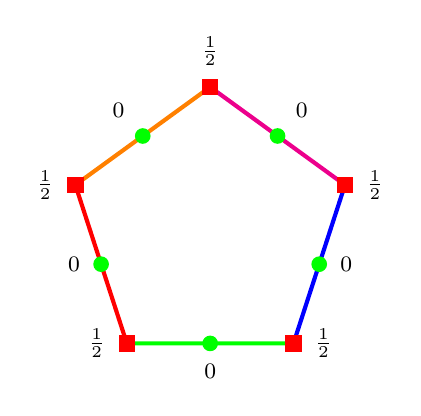
\begin{tikzpicture}  [scale=0.3]

\newdimen\ms
\ms=0.05cm

\tikzstyle{every path}=[line width=1.5pt]


\tikzstyle{s}=[color=red,inner sep=2,rectangle,minimum size=6]
\tikzstyle{c}=[color=green,circle,inner sep=2,minimum size=4]

% Radius of regular polygons
\newdimen\R
\R=6cm     % outer circle

%\r= { \R * sqrt(3) }     % inner circle
%\newdimen\r
%\r=    {\R * sqrt(3)/2}       % inner circle

%\newdimen\K
%\K=3cm

% Define positions of all observables
\path
  ({90 + 0 * 360 /5}:\R      ) coordinate(1)
  ({90 + 36 + 0 * 360 /5}:{\R * sqrt((25+10*sqrt(5))/(50+10*sqrt(5)))}      ) coordinate(2)
  ({90 + 1 * 360 /5}:\R   ) coordinate(3)
  ({90 + 36 + 1 * 360 /5}:{\R * sqrt((25+10*sqrt(5))/(50+10*sqrt(5)))}   ) coordinate(4)
  ({90 + 2 * 360 /5}:\R  ) coordinate(5)
  ({90 + 36 + 2 * 360 /5}:{\R * sqrt((25+10*sqrt(5))/(50+10*sqrt(5)))}  ) coordinate(6)
  ({90 + 3 * 360 /5}:\R  ) coordinate(7)
  ({90 + 36 + 3 * 360 /5}:{\R * sqrt((25+10*sqrt(5))/(50+10*sqrt(5)))}  ) coordinate(8)
  ({90 + 4 * 360 /5}:\R     ) coordinate(9)
  ({90 + 36 + 4 * 360 /5}:{\R * sqrt((25+10*sqrt(5))/(50+10*sqrt(5)))}     ) coordinate(10)
;

% draw contexts

\draw [color=orange] (1) -- (2) -- (3);
\draw [color=red] (3) -- (4) -- (5);
\draw [color=green] (5) -- (6) -- (7);
\draw [color=blue] (7) -- (8) -- (9);
\draw [color=magenta] (9) -- (10) -- (1);    %


%
%%
%% draw atoms
%%
%
\draw (1) coordinate[s,fill=red,label=90:{\footnotesize $\frac{1}{2}$}];   %
%
\draw (2) coordinate[c,fill=green,label={above left:\footnotesize $0$}];    %
%
\draw (3) coordinate[s,fill=red,label={left:\footnotesize $\frac{1}{2}$}]; %
%
\draw (4) coordinate[c,fill=green,label={left:\footnotesize $0$}];  %
%
\draw (5) coordinate[s,fill=red,label={left:\footnotesize $\frac{1}{2}$}];  %
%
\draw (6) coordinate[c,fill=green,label={below:\footnotesize $0$}];
%
\draw (7) coordinate[s,fill=red,label={right:\footnotesize $\frac{1}{2}$}];  %
%
\draw (8) coordinate[c,fill=green,label={right:\footnotesize $0$}];  %
%
\draw (9) coordinate[s,fill=red,label={right:\footnotesize $\frac{1}{2}$}];
%
\draw (10) coordinate[c,fill=green,label={above right:\footnotesize $0$}];  %
%
%
\end{tikzpicture}
\end{center}
\end{frame}

\section{Examples: ``exotic'' probabilities on House/Pentagon/Pentagram hyperdiagram}

\frame{
 \frametitle{Examples: ``exotic'' probabilities on House/Pentagon/Pentagram hyperdiagram}

In this case the conditional probabilities of any two distinct contexts ${\cal C}_i$ and ${\cal C}_j$, for $1\le i,j \le 5$ are
\begin{equation}
\begin{split}
\left[ P( {\cal C}_i \vert {\cal C}_j )\right] \equiv
\begin{bmatrix}
\frac{ 1 }{ 2 }  &  0   &  \frac{ 1 }{ 2 }    \\
0  &  0   &  0  \\
\frac{ 1 }{ 2 }  &  0   &  \frac{ 1 }{ 2 }
\end{bmatrix}
.
\end{split}
\end{equation}

}

\section{Summary}

\frame{
 \frametitle{Summary}

Kolmogorov's axioms of probability theory are extended to conditional probabilities among distinct (and sometimes intertwining) contexts. Formally, this amounts to row stochastic matrices whose entries characterize the conditional probability to find some observable (postselection) in one context, given an observable (preselection) in another context. As the respective probabilities need not (but, depending on the physical/model realization, can) be of the Born rule type, this generalizes approaches to quantum probabilities by Auff\'eves and Grangier, which in turn are inspired by Gleason's theorem.

}



\frame{

\centerline{\Large {\color{magenta} Thank you for your attention!}}

\begin{center}\color{orange}
$\widetilde{\qquad \qquad }$
$\widetilde{\qquad \qquad}$
$\widetilde{\qquad \qquad }$
\end{center}
 }
 \end{document}


















\section{ }

\frame{
 \frametitle{ }

\begin{itemize}
\item[$\bullet$] {
%\color{purple}
}
\pause
\item[$\bullet$] {
%\color{purple}
}
\end{itemize}
}

\section{ }

\frame{
 \frametitle{ }

\begin{itemize}
\item[$\bullet$] {
%\color{purple}
}
\pause
\item[$\bullet$] {
%\color{purple}
}
\end{itemize}
}

\section{ }

\frame{
 \frametitle{ }

\begin{itemize}
\item[$\bullet$] {
%\color{purple}
}
\pause
\item[$\bullet$] {
%\color{purple}
}
\end{itemize}
}

\section{ }

\frame{
 \frametitle{ }

\begin{itemize}
\item[$\bullet$] {
%\color{purple}
}
\pause
\item[$\bullet$] {
%\color{purple}
}
\end{itemize}
}

